%!TeX root=../glasstop.tex
\chapter{Which Dreamed It?}

\lettrine[lines=4,ante=`]{Y}{our} majesty shouldn't purr so loud,' Alice said, rubbing her eyes, and addressing the kitten, respectfully, yet with some severity. »You woke me out of oh! such a nice dream! And you've been along with me, Kitty—all through the Looking-Glass world. Did you know it, dear?«

It is a very inconvenient habit of kittens (Alice had once made the remark) that, whatever you say to them, they \textit{always} purr. »If they would only purr for »yes« and mew for »no,« or any rule of that sort,« she had said, »so that one could keep up a conversation! But how \textit{can} you talk with a person if they always say the same thing?«

On this occasion the kitten only purred: and it was impossible to guess whether it meant »yes« or »no.«

So Alice hunted among the chessmen on the table till she had found the Red Queen: then she went down on her knees on the hearth-rug, and put the kitten and the Queen to look at each other. »Now, Kitty!« she cried, clapping her hands triumphantly. »Confess that was what you turned into!«

(»But it wouldn't look at it,« she said, when she was explaining the thing afterwards to her sister: »it turned away its head, and pretended not to see it: but it looked a \textit{little} ashamed of itself, so I think it \textit{must} have been the Red Queen.«)

»Sit up a little more stiffly, dear!« Alice cried with a merry laugh. »And curtsey while you're thinking what to—what to purr. It saves time, remember!« And she caught it up and gave it one little kiss, »just in honour of having been a Red Queen.«

»Snowdrop, my pet!« she went on, looking over her shoulder at the White Kitten, which was still patiently undergoing its toilet, »when \textit{will} Dinah have finished with your White Majesty, I wonder? That must be the reason you were so untidy in my dream—Dinah! do you know that you're scrubbing a White Queen? Really, it's most disrespectful of you!

And what did \textit{Dinah} turn to, I wonder?« she prattled on, as she settled comfortably down, with one elbow in the rug, and her chin in her hand, to watch the kittens. »Tell me, Dinah, did you turn to Humpty Dumpty? I \textit{think} you did—however, you'd better not mention it to your friends just yet, for I'm not sure.

By the way, Kitty, if only you'd been really with me in my dream, there was one thing you \textit{would} have enjoyed—I had such a quantity of poetry said to me, all about fishes! To-morrow morning you shall have a real treat. All the time you're eating your breakfast, I'll repeat »The Walrus and the Carpenter« to you; and then you can make believe it's oysters, dear!

Now, Kitty, let's consider who it was that dreamed it all. This is a serious question, my dear, and you should \textit{not} go on licking your paw like that—as if Dinah hadn't washed you this morning! You see, Kitty, it \textit{must} have been either me or the Red King. He was part of my dream, of course—but then I was part of his dream, too! \textit{Was} it the Red King, Kitty? You were his wife, my dear, so you ought to know—Oh, Kitty, \textit{do} help to settle it! I'm sure your paw can wait!« But the provoking kitten only began on the other paw, and pretended it hadn't heard the question.

Which do \textit{you} think it was?

\vfill
\centerline{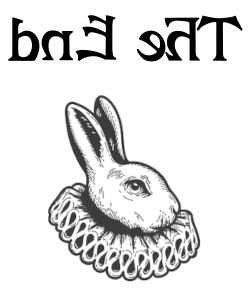
\includegraphics[width=0.4\textwidth]{dne}}
\vfill
\clearpage

\vspace*{\fill}\begin{verse}
A boat beneath a sunny sky,\\
Lingering onward dreamily\\
In an evening of July—

Children three that nestle near,\\
Eager eye and willing ear,\\
Pleased a simple tale to hear—

Long has paled that sunny sky:\\
Echoes fade and memories die.\\
Autumn frosts have slain July.

Still she haunts me, phantomwise,\\
Alice moving under skies\\
Never seen by waking eyes.

Children yet, the tale to hear,\\
Eager eye and willing ear,\\
Lovingly shall nestle near.

In a Wonderland they lie,\\
Dreaming as the days go by,\\
Dreaming as the summers die:

Ever drifting down the stream—\\
Lingering in the golden gleam—\\
Life, what is it but a dream?
\end{verse}
\vfill
\thispagestyle{plain}
